%# -*- coding: utf-8-unix -*-
\chapter{基于波浪干涉效应的理论分析}
\label{chap:analysis}
Kelvin的分析?表明,对于在无限宽广的静水中以速度$V$直线航行的船长为$L$的船,
其远场波形不超过半角为$\psi^K\approx19^\circ28'$的楔形区域。该波系称为
Kelvin波系,$\psi^K$称Kelvin角。然而很多观察?发现,船波有时呈现窄V字形,且V
字形的半角$\psi_\max$显著小于Kelvin角,即$\psi_{\max}<\psi^K$。目前许多理论已被
提出以解释这一``出乎意料''的现象,其中理论?基于定常船波的线性势流理论,
而不像理论?引入复杂的非线性、非定常效应。?提出了``截断波长''假设,即假设船兴波
的波长不超过船长,但未对该假设提出合理的解释。
?提出的两点兴波模型,基于波浪干涉
效应的初等分析,预报的$\psi_\max$的大小与观测结果?一致。本章首先总结基于波浪干涉
效应的两点兴波模型的分析,推导了用两兴波点表示的单体船和双体船最大波高所在的射线
与航迹的夹角$\psi_{\max}$随弗洛德数变化的关系。
然后在线性势流理论的框架下论证了截断波长假设的逻辑漏洞,
并基于两点兴波的相消干涉对长波长散波波高的消除,得到了等效截断波长。结果表明
等效截断波长随弗洛德数变化显著,因此用船长(或其他固定值)作为截断波长是不合理的。

\section{两点兴波模型假设}
\label{sec:2pwavmkr}

第?章介绍了由Kelvin?基于驻相法得出的远场波形,Kelvin波系仅取决于无因次化的
坐标$(x,y)=(X,Y)g/V^2$,这里$g$为重力加速度。另外Kelvin的渐近分析只考虑了
船波的相位而没有(也不能)考虑船波的波高。横波和散波的波高$A^T$和$A^D$强烈地
受到弗洛德数和船体形状的影响,只能通过考虑船体表面边界条件?得到。若干理论和计算方法
可用于满足船体表面条件,得到满足船舶在静水中直航兴波的边值问题?的完全解,
如NK理论?、薄船理论?、NM理论?以及Hogner近似?。
然而,考虑到船的主要兴波产生于船体形状变化最迅速的地方---船首和船尾,实际上
不求解上述边值问题也可得到关于幅值$A^T$和$A^D$的有用见解。

单体船产生的远场波可看作两分别起源于``实效船首''$x^b$和``实效船尾''$x^s$的Kelvin波系
的叠加。这里$x^b\equiv X^b/L$代表首波位于首柱后的波峰的位置,而$x^s\equiv X^s/L$代表
尾波的第一个波谷的位置。其间距$\ell\equiv (X^b-X^s)/L=x^b-x^s$,
工程上常用$\ell=0.9$代表这段距离。船首和船尾产生的两Kelvin波系的叠加如图?所示。
现在,叠加的波系取决于船长$L$,定义Froude数
\begin{equation}
  F\equiv V/\sqrt{gL}
  \label{eq:Fdef}
\end{equation}
现在考虑由完全相同的相距$S$的两片体组成的双体船的远场波。
为了方便分析,忽略船尾的兴波。双体船产生的远场波可看作两起源于两片体船首
$(0,\pm s/2)$的Kelvin波系的叠加,这里$s\equiv S/L$是无因次化的片体间距。
定义Froude数
\begin{equation}
  F_s\equiv V/\sqrt{gS}
  \label{eq:Fsdef}
\end{equation}
由定义可知$F_s=F/\sqrt{s}$。两片体船首产生的两Kelvin波系的叠加如图?所示。

\section{基本关系}
\label{sec:basicralations}

由第?章可知,在离开船体一小段距离之后,船波可用一系列传播方向与航行成
$\pi/2<\gamma<\pi/2$角度的基本波的叠加表示。这些基本波是满足
下半平面$z<0$内的Laplace方程?,未扰动的自由面$z=0$上的线性自由面边界条件?,
和深水边界条件?的本征解。这些解可表示为
\begin{equation}
  \mathrm{e}^{kz+\mathrm{i}k(\cos\gamma+\sin\gamma)}
  \label{eq:eigensolution}
\end{equation}
其中波数$k$和传播方向$\gamma$满足色散关系
\begin{equation}
  F^2k=1+\tan^2\gamma
  \label{eq:disperploar}
\end{equation}

在远场$h\equiv\sqrt{x^2+y^2}\to\infty$,由驻相法可知,
对基本波\eqref{eq:eigensolution}的叠加中贡献最大的基本波的相位
\begin{equation}
  \theta\equiv(x\cos\gamma+y\sin\gamma)(1+\tan^2\gamma)/F^2
  \label{eq:phasepolar}
\end{equation}
是稳定的,也即传播方向$\gamma$是``驻相关系'' $d\theta/d\gamma=0$的根。由此可得,
\begin{equation}
  \tan\psi\equiv\frac{y}{-x}=\frac{\tan\gamma}{1+2\tan^2\gamma}
  \label{eq:statfazploar}
\end{equation}

\section{单体船兴波特征}
\label{sec:monowavchar}
兴波显著的实效船首$x=x^b$和实效船尾$x=x^s$间的距离$\ell$在波浪传播方向
$(\cos\gamma,\sin\gamma)$上的投影为$\ell\cos\gamma$。相长干涉的发生需要满足条件
\begin{equation}
  \ell\cos\gamma=(2n-1)\lambda/2\equiv(2n-1)\pi F^2\cos^2\gamma,\quad n\ge 1
  \label{eq:unfavorintrf}
\end{equation}
由式\eqref{eq:unfavorintrf}可得$1/\cos\gamma=(2n-1)\pi F^2/\ell$或者
\begin{equation}
  \tan^2\gamma=(2n-1)^2\pi^2F^4/\ell^2-1,\quad n\ge1
  \label{eq:xintrfrelation}
\end{equation}
这是分布在船首和船尾的两个兴波点的兴波的相长干涉条件。

由第?章的分析可知,横波对应的传播方向为$0\le\tan^2\gamma\le 1/2$。此关系式和式
\eqref{eq:xintrfrelation}表明单体船首尾横波的相长干涉的发生范围是
\begin{equation}
  \sqrt{\ell/\pi}\approx0.535\le\sqrt{2n-1}F\le(3/2)^{1/4}\sqrt{\ell/\pi}
  \approx0.59,\quad n\ge 1
  \label{eq:xintrfrange}
\end{equation}

设计船舶时需要避免波长最大的首尾横波间的相长干涉,而波长最大的波的传播方向为
$\gamma=0$,即沿船的航向。因此由式\eqref{eq:xintrfrange}可知,波长最大的首尾
横波的相长干涉发生在一系列弗洛德数
\begin{equation}
  F_n^T\equiv\sqrt{\ell/\pi}/\sqrt{2n-1}\approx 0.535,0.31,0.24,0.20,\cdots
  \label{eq:FnT}
\end{equation}
这些Froude数$F_n^T$必须在设计时加以避免。一般地,式\eqref{eq:xintrfrange}
定义了首尾横波相长干涉发生的一系列Froude数区间
\begin{equation}
  \cdots,0.20\le F\le0.224, \quad 0.24\le F\le 0.265,\quad 0.31\le F\le 0.34,
  \quad 0.535\le F\le 0.59
  \label{FnTrange}
\end{equation}

在实践中,船舶设计师使用类似但比式\eqref{eq:xintrfrange}更精确的公式来
设计船舶使首尾横波发生相消干涉,该公式引入棱形系数来考虑船体形状的影响。

散波对应的传播方向为$\tan^2\gamma^2\ge 1/2$。此关系式和式\eqref{eq:xintrfrelation}
表明单体船首尾散波的相长干涉的发生范围是
\begin{equation}
  (3/2)^{1/4}\sqrt{\ell/\pi}\approx 0.59\le\sqrt{2n-1}F,\quad n\ge 1
  \label{eq:xdivintrfrange}
\end{equation}
由干涉条件\eqref{eq:xintrfrelation}和驻相关系\eqref{eq:statfazploar}可得
\begin{equation}
  \tan\psi_n=\frac{\sqrt{(2n-1)^2\pi^2F^4/\ell^2-1}}{2(2n-1)^2\pi^2F^4/\ell^2-1}
  \label{eq:psixn}
\end{equation}
由式\eqref{eq:psixmax}可知当$F>F_n^K$时,$\psi_n\le\psi^K$,其中
\begin{equation}
  F_n^K\equiv (3/2)^{1/4}\sqrt{\ell/\pi}/\sqrt{2n-1}
  \label{eq:Fxn}
\end{equation}

令式\eqref{eq:psixn}和\eqref{eq:Fxn}中$n=1$可得
\begin{equation}
  \tan\psi^x_{\max}=\frac{\sqrt{\pi^2F^4/\ell^2-1}}{2\pi^2F^4/\ell^2-1}
  \quad\text{当}\quad F\ge F^x\equiv (3/2)^{1/4}\sqrt{\ell/\pi}\approx 0.59
  \label{eq:psixmax}
\end{equation}
式\eqref{eq:psixmax}表明,$\psi^x_{\max}\le\psi^K$当$F\ge F^K$。
因此,当$F=F^K\approx0.59$时,由散波的相长干涉产生的波高最大的波位于Kelvin臂上,
而当$F>F^K$时,波高最大的波位于Kelvin尾迹内。

图\ref{fig:psilongintrf}是$1\le n\le4$时船首波和尾波相长干涉产生的最大波高
的尾流角度$\psi_n$,由式
\eqref{eq:psixn}定义。其中,由横波和散波造成的干涉分别用虚线和实线表示。
图中虚线和实线的连接点处最大波高位于Kelvin臂上,其对应的Froude数由式
\eqref{eq:Fxn}定义。图\ref{fig:psilongintrf}还显示了\parencite{Rabaud2013Ship}
的观测结果。图\ref{fig:psilongintrf}表明,散波干涉产生的最大波高位置与
$0.6<F<1.2$范围内的观测结果随Froude数的变化趋势一致。此外,由式\eqref{eq:psixn}
可知,$F=0.453$时$\psi_2\approx 13^\circ$,$F=0.544$时$\psi_1\approx13^\circ$。
图\ref{fig:psilongintrf}表明,这两个值与$F\approx 0.5$时的观测结果
$\psi_{\max}\approx 13^\circ$一致,
而这两个值分别对应$n=2$时散波的相长干涉和$n=1$时横波的相长干涉。因此,单体船
首尾散波的干涉是$0.6<F<1.2$时观测到半角明显小于Kelvin角的窄V字形尾迹的可信解释。
而$F<0.6$时观测到的窄V字形尾迹可以用单体船首尾散波和首尾横波的干涉解释。
%
\begin{figure}[htp]
  \centering
  \captionstyle{\centering}
  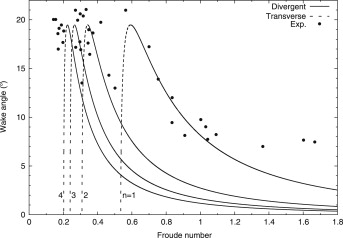
\includegraphics[width=0.5\textwidth]{chap3/psilongintrf.jpg}
  \bicaption[fig:psilongintrf]{单体船首尾波系干涉产生的波高最大的波的尾流角度}
  {单体船首尾散波(实线)或首尾横波(虚线)相长干涉造成的波高最大的波的尾流角度}{Fig}{Ray angles $\psi_n$ defined by \eqref{eq:psixn} with $1\le n\le 4$ along which divergent or transverse waves are
largest due to interference between the divergent (solid lines) or transverse
(dashed lines) waves created by the bow and the stern of a monohull ship}
\end{figure}

\section{双体船兴波特征}
\label{sec:catwavchar}

双体船两片体间距$s$在波浪传播方向$(\cos\gamma,\sin\gamma)$上的投影长度为
$s\sin\gamma$。由两片体首部产生的横波或散波间的相长干涉的发生条件为
\begin{equation}
  s\sin\gamma=n\lambda\equiv 2n\pi F^2\cos^2\gamma,\quad n\ge 1
  \label{eq:yunfavorintrf}
\end{equation}
由干涉条件\eqref{eq:yunfavorintrf}和式\eqref{eq:Fsdef}得
$\tan\gamma/\cos\gamma=2n\pi F_s^2$或者
\begin{equation}
  (1+\tan^2\gamma)\tan^2\gamma=4n^2\pi^2F_s^4
  \label{eq:yintrfrelation}
\end{equation}
由式\eqref{eq:yintrfrelation}和驻相关系\eqref{eq:statfazploar}可知
\begin{equation}
  \tan\psi_n^y=\sqrt{\frac{\sqrt{1+16n^2\pi^2F_s^4}-1}{2+32n^2\pi^2F_s^4}}
  \label{eq:psiyn}
\end{equation}
当Froude数$F_s=F_n^y$时,$\psi_n^y$等于Kelvin角$\psi^K$
\begin{equation}
  F_n^y=\frac{3^{1/4}}{2\sqrt{n\pi}}
  \label{eq:Fsn}
\end{equation}
由\eqref{eq:Fsn}可知
\begin{equation}
  F_1^y\equiv F_s^y\approx 0.37,\quad F_2^y\approx0.26,\quad F_3^y\approx 0.214,
  \quad F_4^y\approx 0.19, \cdots
\end{equation}
横波的相长干涉对应$0<F_s\le F_n^y$,而散波的相长干涉对应$F_s\ge F_n^y$。

令式\eqref{eq:psiyn}中$n=1$得
\begin{equation}
  \tan\psi_{\max}^y=\sqrt{\frac{\sqrt{1+16\pi^2F_s^4}-1}{2+32\pi^2F_s^4}}
  \label{eq:psiymax}
\end{equation}

图\ref{fig:psilatintrf}是$1\le n\le4$时双体船两片体产生的首波间相长干涉
造成的最大波高的尾流角度$\psi_n^y$,由式\eqref{eq:psiyn}定义。
其中,由横波和散波造成的干涉分别用虚线和实线表示。图中实线和虚线的连接点处
最大波高位于Kelvin臂上,其对应的Froude数由式\eqref{eq:Fsn}定义。图中还显示了
\parencite{Rabaud2013Ship}报告的处于$1.3<F<1.8$的观测数据。图\ref{fig:psilatintrf}
的横坐标是$F_s=F/\sqrt{s}$,而\parencite{Rabaud2013Ship}并未给出与观测数据对应的
船是单体船还是双体船。为了进行对比,假定处于$1.3<F<1.8$范围内的船是双体船,且片体
间距为$s=1$。从图\ref{fig:psilatintrf}可见,$1.3<F<1.8$范围内的观测数据与
双体船两片体首部区域产生的散波间的相长干涉产生的最大波高的尾流角$\psi_{\max}^y$
一致。
%
\begin{figure}[htp]
  \centering
  \captionstyle{\centering}
  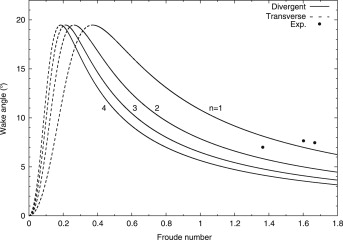
\includegraphics[width=0.5\textwidth]{chap3/psilatintrf.jpg}
  \bicaption[fig:psilatintrf]{双体船两片体首波系干涉产生的波高最大的波的尾流角度}
  {双体船两片体首部产生的散波(实线)或横波(虚线)干涉造成的波高最大的波的尾流
  角度}{Fig}
  {Ray angles $\psi_n^y$ defined by \eqref{eq:psiyn} with $1\le n\le 4$ 
  along which divergent or transverse waves are
largest due to interference between the divergent (solid lines) or transverse
(dashed lines) waves created by the bows of the twin hulls of a catamaran}
\end{figure}

\section{截断波长假设的逻辑漏洞}
\label{sec:cutoffwavlen}

由式\eqref{eq:disperploar}给出的色散关系$F^2k=1/\cos^2\gamma$可知波长
$\lambda=2\pi/k$可以表示为
\begin{equation}
  \lambda=2\pi F^2\cos^2\gamma\le 2\pi F^2\equiv \lambda^{\max}
  \label{eq:wavlenchap3}
\end{equation}
因此,船产生的最大波长$\lambda^{\max}$在$F<1/\sqrt{2\pi}\approx0.4$时小于船长,
在$F>0.4$时大于船长,正如众所周知的和第?章给出的。

由驻相关系\eqref{eq:disperploar}和式\eqref{eq:wavlenchap3}可知波长为$\lambda$
的尾流角度$\psi$是
\begin{equation}
  \tan\psi=\frac{\sqrt{\lambda^{max}/\lambda}-1}{2\lambda^{max}/\lambda-1}
  \equiv\frac{\sqrt{\lambda'(1-\lambda')}}{2-\lambda'}
  \quad\text{其中}\quad \lambda'=\lambda/\lambda^{\max}
  \label{eq:psiwavlen}
\end{equation}
由式\eqref{eq:psiwavlen}定义的$\psi$对$0\le\lambda'\le1$是实数。
当$0\le\lambda'\le2/3$时$\psi$从0增加到$\psi^K$,而当$2/3\le\lambda'\le1$时
$\psi$从$\psi^K$减小到0,如图\ref{fig:psiwavlen}所示。短波$0\le\lambda'\le 2/3$
和长波$2/3\le\lambda'\le 1$分别对应Kelvin波系中的散波和横波。
%
\begin{figure}[htp]
  \centering
  \captionstyle{\centering}
  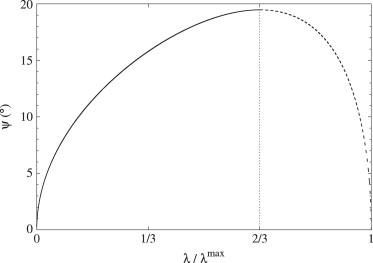
\includegraphics[width=0.5\textwidth]{chap3/psiwavlen.jpg}
  \bicaption[fig:psiwavlen]{尾流角度$\psi$随$\lambda/\lambda^{\max}$的变化}
  {当波长在$0\le\lambda/\lambda^{\max}\le1$范围内变化时,对应的尾流角度的变化}{Fig}
  {Variation of the corresponding ray angle $\psi$ for $0\le\lambda/\lambda^{\max}
\le1$}
\end{figure}

位于Kelvin臂$\psi=\psi^K$的波浪的波长为
\begin{equation}
  \lambda^{cusp}=2\lambda^{\max}/3=4\pi F^2/3
  \label{eq:wavlencusp}
\end{equation}
由式\eqref{eq:wavlencusp}可见,当$F<\sqrt{3/\pi}/2\approx0.49$时,Kelvin臂处的波长
$\lambda^{cusp}$小于船长,而当$F>0.49$时则大于船长。
现在我们只考虑$0\le\lambda\le\lambda^{cusp}$范围内的波浪,即散波。
由式\eqref{eq:psiwavlen}可知,尾流角度$\psi$上的散波的波长$\lambda^D$为
\begin{equation}
  \frac{\lambda^D}{\lambda^{\max}}}\equiv\frac{8\tan^2\psi}{1+4\tan^2\psi+
    \sqrt{1-8\tan^2\psi}}
  \label{eq:wavlendiv}
\end{equation}

对于散波$0\le\lambda\le\lambda^{cusp}$来说,由式\eqref{eq:psiwavlen}定义的函数
$\psi(\lambda)$是增函数。因此下面的不等式
\begin{eqnarray}
  &&\lambda\le\lambda^{cut}\quad\text{和} \label{eq:wavlenneq}\\
  &&\psi\le\psi^{cut}\equiv\arctan\left(
  \frac{\sqrt{\lambda^{max}/\lambda^{cut}-1}}{2\lambda^{max}/\lambda^{cut}-1}
  \right)
  \label{eq:psineq}
\end{eqnarray}
在数学上是等价的,其中$\lambda^{cut}\le\lambda^{cusp}$,$\psi^{cut}\le\psi^K$。
令式\eqref{eq:psineq}中$\lambda^{cut}=1$,即假设船波的波长不超过船长\supercite{Rabaud2013Ship},并将$\lambda^{\max}=2\pi F^2$代入,可得
\begin{equation}
  \tan\psi_{\max}=\frac{\sqrt{2\pi F^2-1}}{4\pi F^2-1}
  \label{eq:rabaudformula}
\end{equation}
式\eqref{eq:rabaudformula}即是\parencite{Rabaud2013Ship}预报的窄V字形尾迹的半角。

式\eqref{eq:wavlenneq}和式\eqref{eq:psineq}在数学上是等价的这一事实意味着,
假定$\lambda<\lambda^{cut}$也就自动将兴波角度$\psi$限制在Kelvin角$\psi^K$内,
因此无异于强制要求$\psi^{cut}\le\psi^K$。显然,引入截断波长假定的模型
(如\parencite{Rabaud2013Ship})无法解释观测到的窄V字形尾迹,除非假定的截断波长
$\lambda^{cut}$能够被证明是合理的。


\section{与最大波高对应的波长}
\label{sec:wavlen}

基于单体船首尾波系的相长干涉或双体船片体间首波系的相长干涉可以给出截断波长
$\lambda^{cut}$的一个合理定义。由前面的分析可知,单体船首尾散波系的相长干涉
会在尾流角度$\psi^x_{\max}$处产生波高最大的波,而双体船片体间首波系的相长干涉
会在尾流角度$\psi^y_{\max}$处产生波高最大的波。尾流角度$\psi^x_{\max}$和
$\psi^y_{\max}$分别由式\eqref{eq:psixmax}和\eqref{eq:psiymax}给出。
在$\psi^x_{\max}\le\psi\le\psi^K$或$\psi^y_{\max}\le\psi\le\psi^K$范围内的波浪
受干涉作用影响,波高小于$\psi^x_{\max}$或$\psi^y_{\max}$上波浪的波高,而由散波
波长$\lambda^D$和尾流角度$\psi$的关系可知,这些范围内的波浪波长大于$\psi^x_{\max}$
或$\psi^y_{\max}$上的波长。 因此波浪干涉作用抑制了波长大的散波的波高。
令式\eqref{eq:wavlendiv}中$\psi=\psi_{\max}$,得到对应$\psi_{\max}$和
基于波浪干涉作用的截断波长$\lambda^{cut}$
\begin{equation}
  \lambda^{cut}\equiv\frac{16\pi F^2\tan^2\psi_{max}}{1+4\tan^2\psi_{\max}+\sqrt{1-8\tan^2\psi_{\max}}}\approx 8\pi F^2\tan^2\psi_{\max}
  \label{eq:wavlencut}
\end{equation}

与单体船首尾波系的干涉和$\psi^x_{\max}$对应的截断波长可由\eqref{eq:psixmax}
和\eqref{eq:wavlencut}求得。由\eqref{eq:psixmax}和\eqref{eq:wavlencut}可知,
当$F\to\infty$时$\lambda^{cut}$的衰减形式为$1/F^2$。

与双体船片体间首波系的干涉和$\psi^y_{\max}$对应得截断波长可由\eqref{eq:psiymax}
和\eqref{eq:wavlencut}求得。由\eqref{eq:psiymax}和\eqref{eq:wavlencut}可知,
当$F\to\infty$时$\lambda^{cut}\to s$。

图\ref{fig:wavlencut}显示了单体船和片体间距为$s=0.1$,0.5,1和1.5的双体船对应的
截断波长$\lambda^{cut}$。当Froude数$F>1.2$时,双体船的截断波长几乎不随$F$变化,
且可以近似为$\lambda^{cut}\approx s$。
因此,假定截断波长是不随Froude变化的常数对双体船而言是合理的。
单体船的截断波长$\lambda^{cut}$是随Froude数$F$迅速衰减的函数,
因此,假定单体船的截断波长是不随Froude数变化的常数是不合理的。
所以,\parencite{Rabaud2013Ship}中的关键性假设$\lambda\le1$不能通过基于波浪干涉
的两点兴波模型得到的结果合理化。
%
\begin{figure}[htp]
  \centering
  \captionstyle{\centering}
  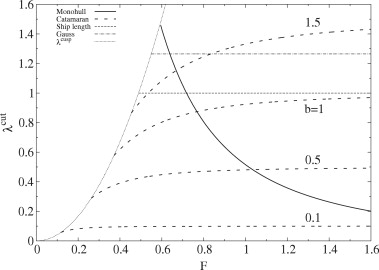
\includegraphics[width=0.5\textwidth]{chap3/wavlencut.jpg}
  \bicaption[fig:wavlencut]
  {单体船和双体船截断波长的变化}
  {与单体船首尾波系干涉和$s=0.1$,0.5,1和1.5的双体船片体间首波系干涉相关的
    截断波长$\lambda^{cut}$随Froude数$F$的变化}
  {Fig}{Variations of the cutoff wavelengths $\lambda^{cut}$ related to
  longitudinal interference between the divergent waves created by the bow
  and the stern of a monohull ship (Monohull) or to lateral interference
  between the divergent waves created by the twin hulls of a catamaran (catamaran)
with $s=0.1$, 0.5, 1 and 1.5}
\end{figure}


\section{本章小结}
\label{sec:analyssum}
本章首先总结了基于波浪干涉效应的两点兴波模型的分析。
由两点兴波模型预测的单体船首波和尾波间的相长干涉或双体船两片体产生的首波间的相长
干涉造成的波高最大的波浪的尾流角度与\parencite{Rabaud2013Ship}观测到的窄V字形尾迹
的半角一致。具体来说,图\ref{fig:psilongintrf}和图\ref{fig:psilatintrf}表明
\parencite{Rabaud2013Ship}的观测数据中Froude数小于或大于1.2的兴波角度分别与
单体船或双体船波高最大的波浪的尾流角度一致。因此波浪干涉是解释窄V字形船尾迹的
可信理论。
本章接着在线性势流理论的框架下对\parencite{Rabaud2013Ship}提出的截断波长假设
进行了批判性的分析。图\ref{fig:wavlencut}表明,截断波长$\lambda^{cut}$
与Froude数无关并约等于船长的假设\supercite{Rabaud2013Ship}无法用基于波浪干涉效应的
两点兴波模型\supercite{Noblesse2014Why}的分析合理化。
